\section{Design}

\subsection{ANTLR}
\begin{frame}
\frametitle{ANTLR}

We use ANTLR to generate a parse tree and walk the parse tree to \emph{collect software quality metrics}.

\begin{definition}
ANTLR (ANother Tool for Language Recognition) is a powerful parser generator for reading, processing, executing, or translating structured text or binary files. (Parr, 2013)
\end{definition}

It can \emph{support multiple programming languages}, as long as you define the language structure using a grammar file\footnote{Open source grammar files: https://github.com/antlr/grammars-v4}.

\end{frame}

\subsection{Architecture for Measurement Component}
\begin{frame}[allowframebreaks]
\frametitle{Architecture for Measurement Component}
Washizaki et al. (2007) proposed a framework that achieves effective measurement and evaluation of source code quality.

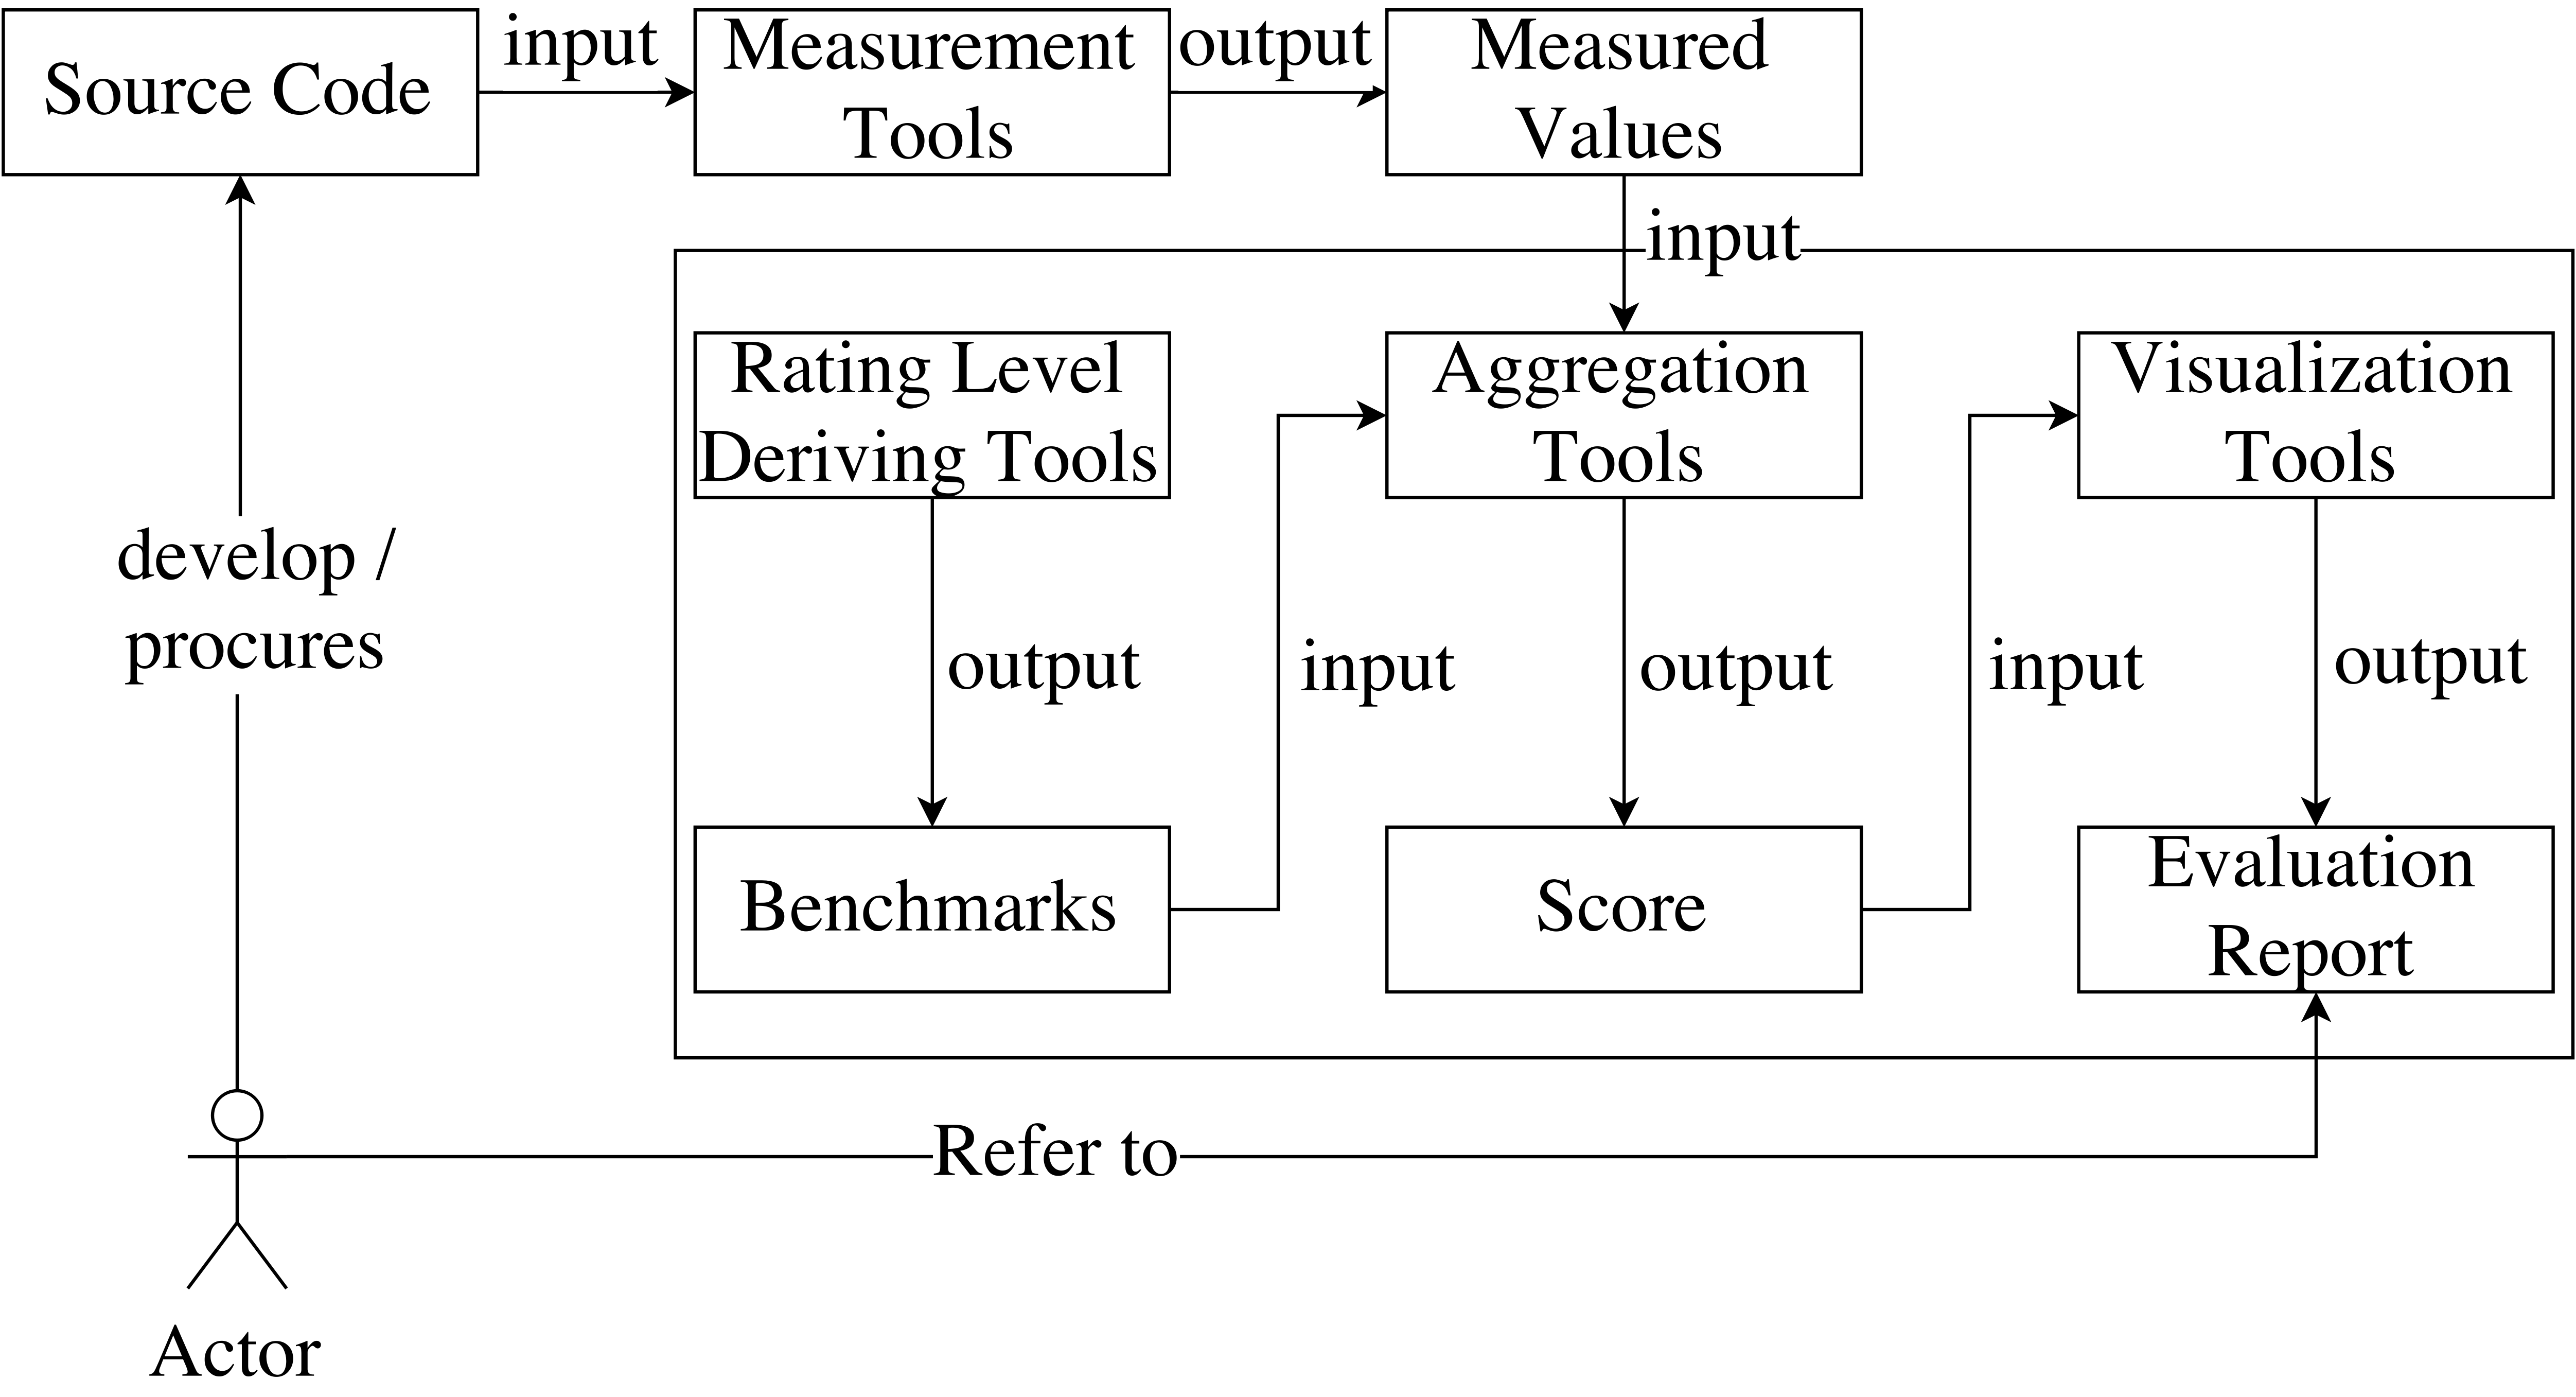
\includegraphics[scale=0.06]{washizaki_framework}

\framebreak

We use the proposed framework to build the measurement component of SQAT.

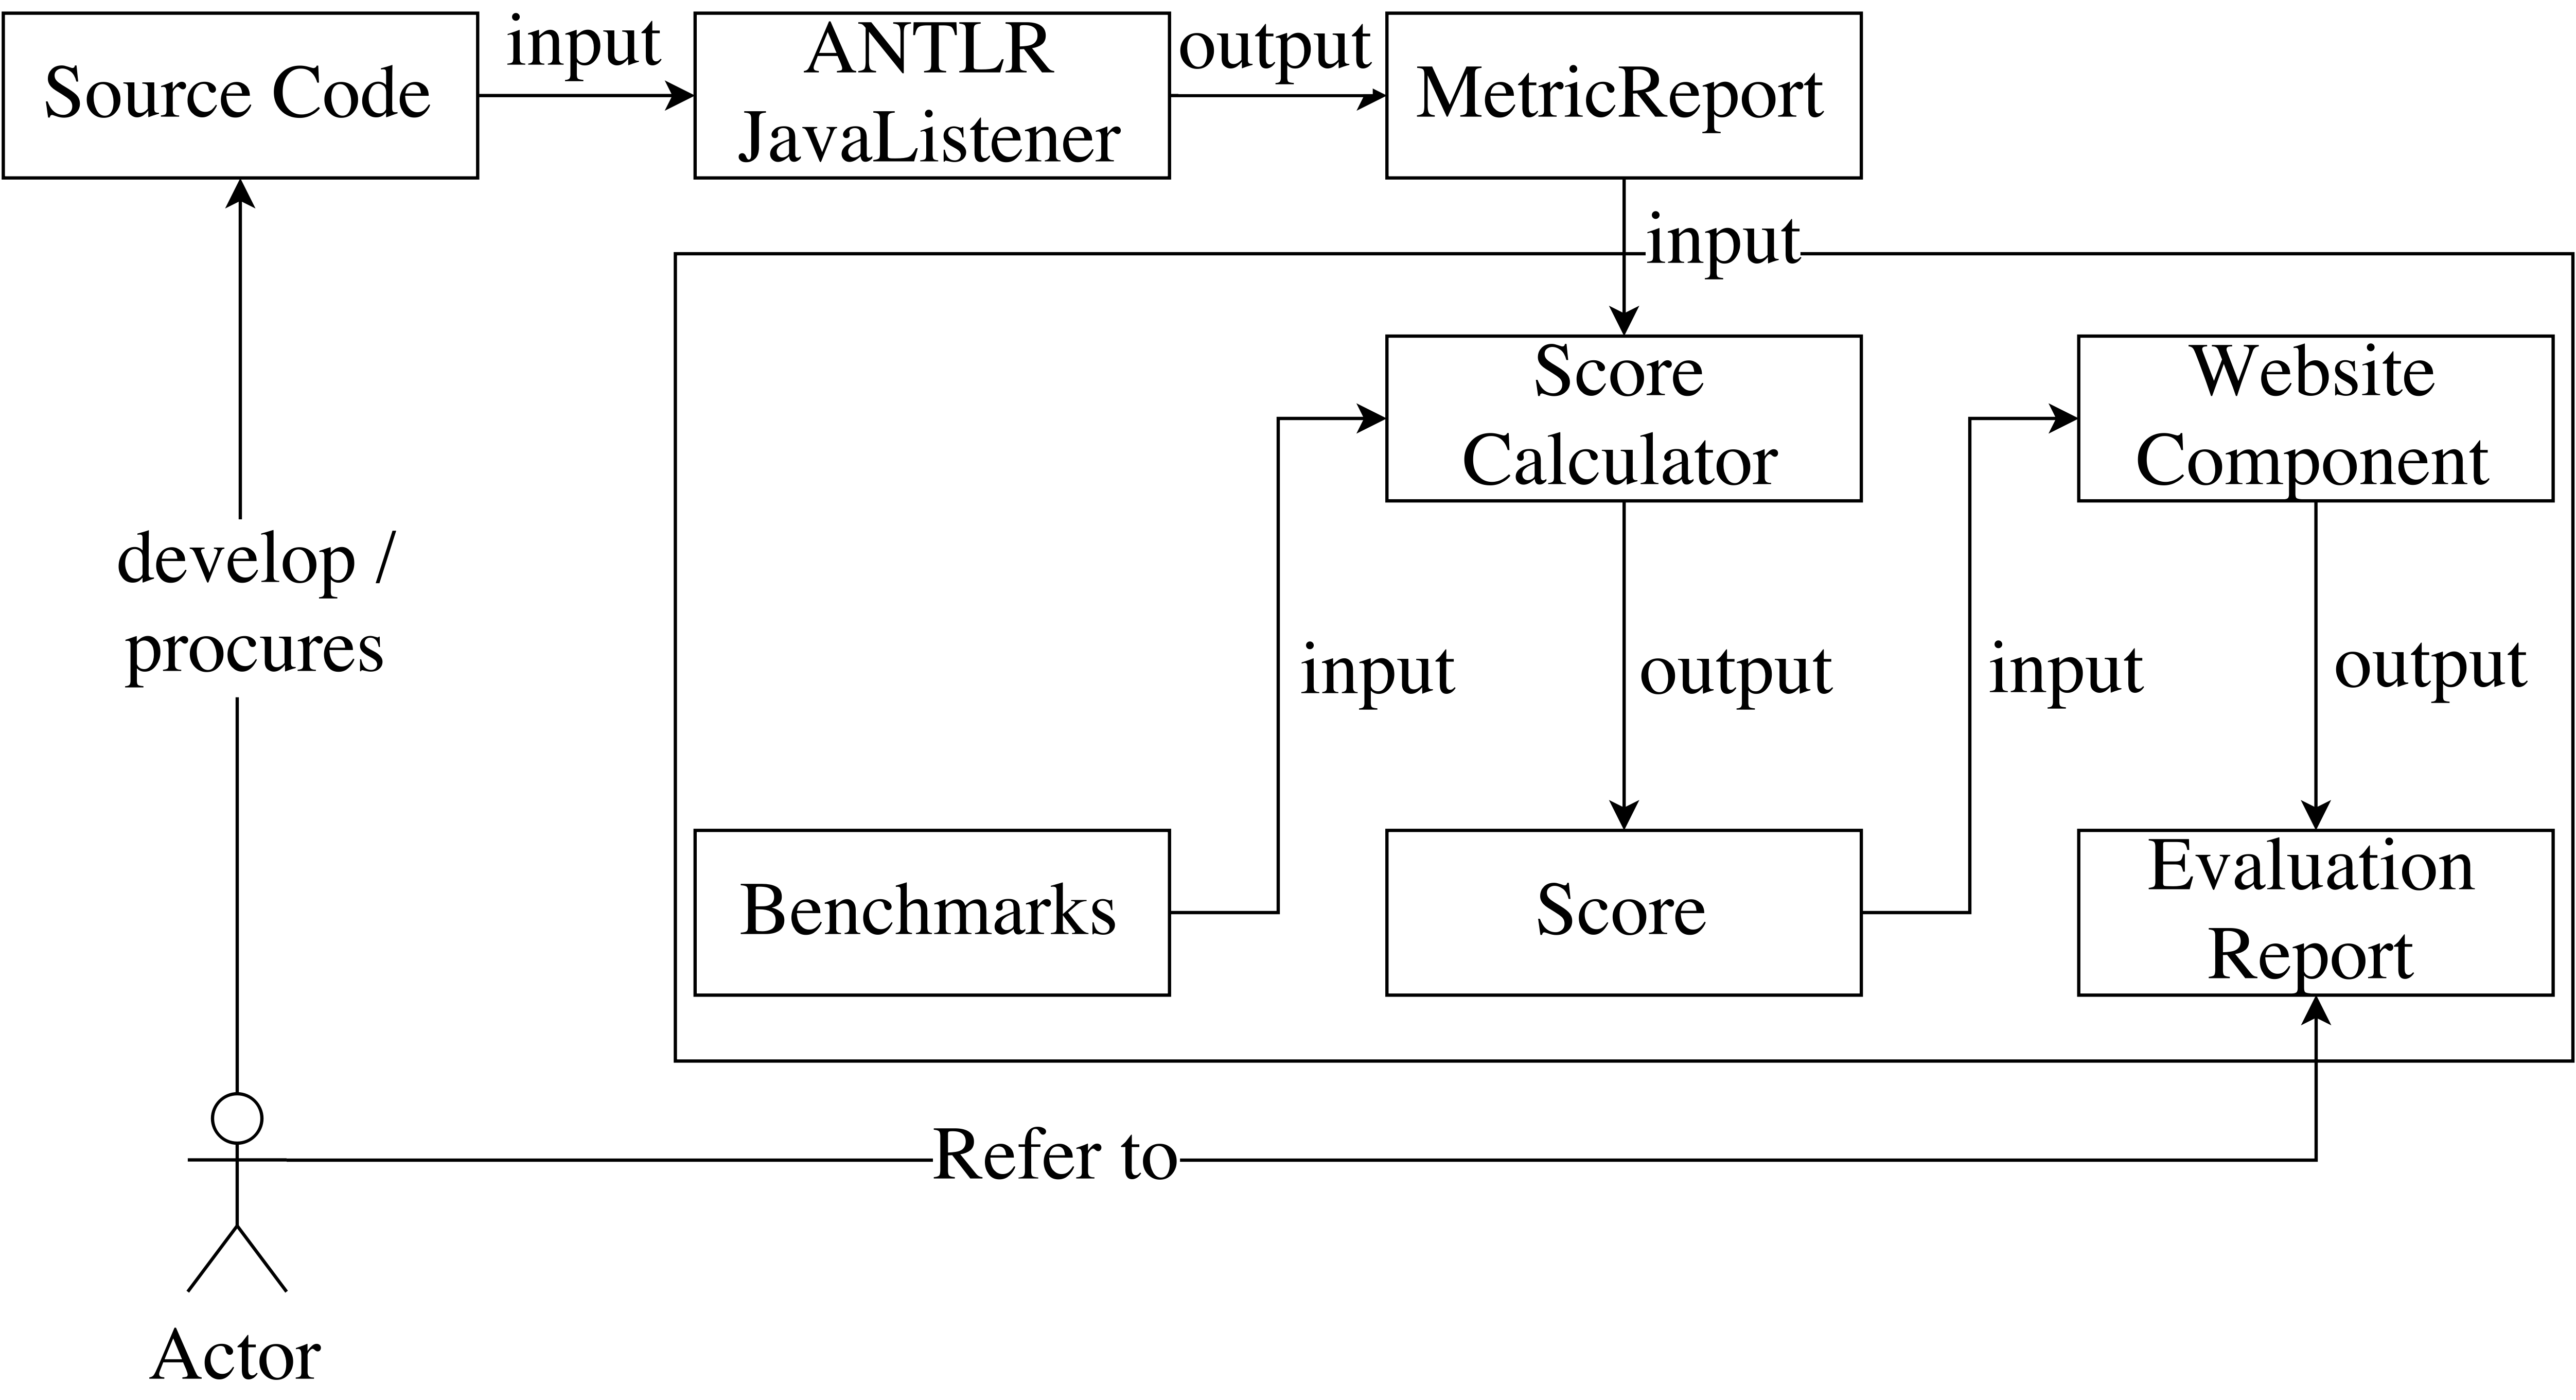
\includegraphics[scale=0.06]{software_quality_measurement_framework}
\end{frame}

\subsection{Overall Architecture}
\label{subsection:overall_architecture}
\begin{frame}[allowframebreaks]
\frametitle{Overall Architecture: Microservices}

\begin{definition}
Microservices is a software architecture style in which complex applications are composed of small, independent processes communicating with each other using language-agnostic API (Fowler, 2014).
\end{definition}

The architecture has three advantages:
\begin{itemize}
  \item Programming language agnostic
  \item Easy to understand due to abstraction at service level
  \item Easy to scale application horizontally
\end{itemize}

\hyperlink{appendix:monolithic}{\beamerbutton{Monolithic Architecture}}

\framebreak

\begin{center}
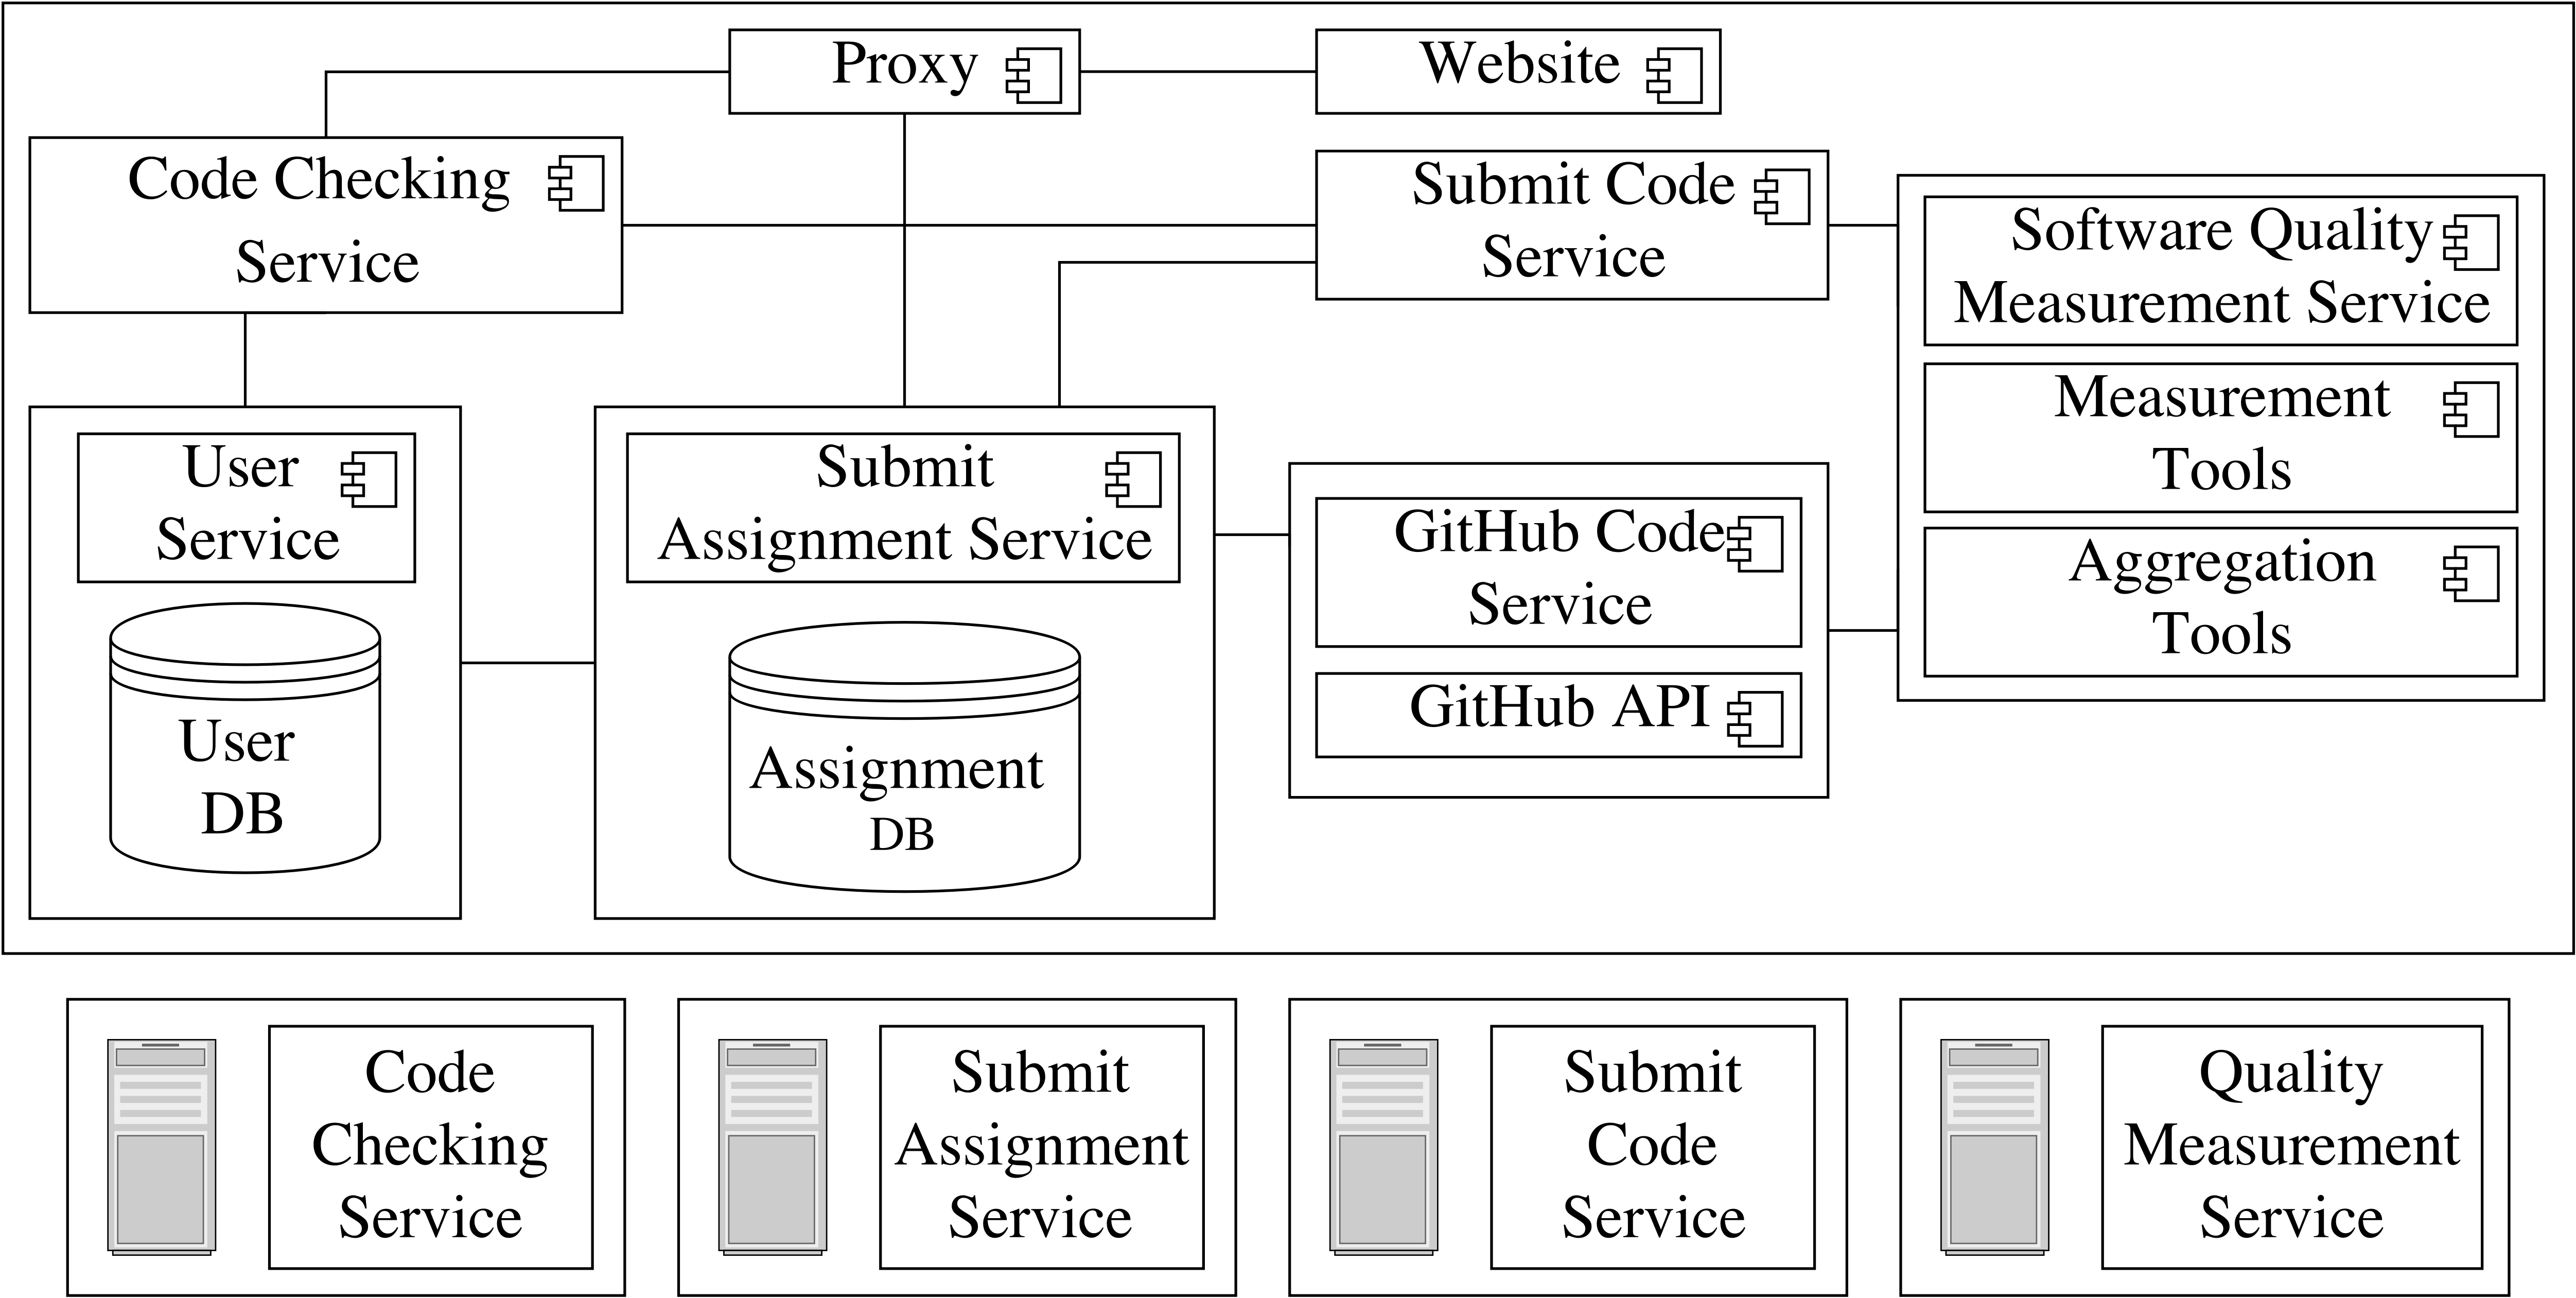
\includegraphics[scale=0.06]{microservice_architecture}
\end{center}
\end{frame}